%%%%%%%%%%%%%%%%%%%%%%%%%%%%%%%%%%%%%%%%%%%%%%%%%%%%%%%%%%%%%%%%%%%%%%%%%%%%%
%%%
%%% File: thesis.tex, version 1.9, May 2016
%%%
%%% =============================================
%%% This file contains a template that can be used with the package
%%% cs.sty and LaTeX2e to produce a thesis that meets the requirements
%%% of the Computer Science Department from the Technical University of Cluj-Napoca
%%%%%%%%%%%%%%%%%%%%%%%%%%%%%%%%%%%%%%%%%%%%%%%%%%%%%%%%%%%%%%%%%%%%%%%%%%%%%

\documentclass[12pt,a4paper,twoside]{report}         
\usepackage{cs}              
\usepackage{times}
\usepackage{graphicx}
\usepackage{latexsym}
\usepackage{amsmath,amsbsy}
\usepackage{amssymb}
\usepackage[matrix,arrow]{xy}
\usepackage[T1]{fontenc}
\usepackage{ae,aecompl}
\usepackage{romanian} %definitii pentru diacritice; 
\usepackage{amstext}
\usepackage{graphics}
\usepackage[T1]{fontenc}
\usepackage{ae,aecompl}
\usepackage{algorithm}
%\usepackage{algorithmic}
\usepackage{color}
\usepackage{color}

% \mastersthesis
\diplomathesis
% \leftchapter
\centerchapter
% \rightchapter
\singlespace
% \oneandhalfspace
% \doublespace

\renewcommand{\thesisauthor}{Alin Dan 'TANDEA}    %% Your name.
\renewcommand{\thesismonth}{Iunie}     %% Your month of graduation.
\renewcommand{\thesisyear}{2018}      %% Your year of graduation.
\renewcommand{\thesistitle}{Managementul studiilor clinice bazat pe
tehnologia blockchain} % Title
\renewcommand{\thesissupervisor}{asis. Ing. Cosmina Ivan}
\newcommand{\department}{FACULTATEA DE AUTOMATIC'A 'SI CALCULATOARE\\
DEPARTAMENTUL CALCULATOARE}
\newcommand{\thesis}{LUCRARE DE LICEN'T'A}
\newcommand{\uline}[1]{\rule[0pt]{#1}{0.4pt}}
%\renewcommand{\thesisdedication}{P'arin'tilor mei}
\newcommand{\utcnlogo}{
\includegraphics[width=15cm]{img/utcn.jpg}}

\begin{document}
%\frontmatter
%\pagestyle{headings}

\newenvironment{definition}[1][Defini'tie.]{\begin{trivlist}
\item[\hskip \labelsep {\bfseries #1}]}{\end{trivlist}}



%\thesistitle                    %% Generate the title page.
%\authordeclarationpage                %% Generate the declaration page.

\pagenumbering{arabic}
\setcounter{page}{4}



\begin{center}
%\includegraphics[width=15cm]{img/tucn.jpg}  
\utcnlogo

{\bf \department}

\vspace{4cm}

{\bf \thesistitle} %LICENSE THESIS TITLE}

\vspace{1.5cm}

\thesis

\vspace{6cm}

Absolvent: {\bf \thesisauthor} 

Conduc'ator 'stiin'tific: {\bf \thesissupervisor}

\vspace{3cm}
{\bf \thesisyear}
\end{center}

\thispagestyle{empty}
\newpage

\begin{center}
\utcnlogo

{\bf \department}
\end{center}
\vspace{0.5cm}

%\begin{small}
\begin{tabular}{p{7cm}p{8cm}}
 %\hspace{-1cm}& VIZAT,\\
 \hspace{-1cm}DECAN, & DIRECTOR DEPARTAMENT,\\
\hspace{-1cm}{\bf Prof. dr. ing. Liviu MICLEA} & {\bf Prof. dr. ing. Rodica POTOLEA}\\  
\end{tabular}
 
\vspace{2cm}

\begin{center}
Absolvent: {\bf \thesisauthor}

\vspace{1cm}

{\bf \thesistitle}
\end{center}

\vspace{1cm}

\begin{enumerate}
 \item {\bf Enun'tul temei:} {\it Scurt'a descriere a temei lucr'arii de licen't'a 'si datele ini'tiale}
\item {\bf Con'tinutul lucr'arii:} {\it (enumerarea p'ar'tilor componente) Exemplu: Pagina de prezentare, aprecierile coordonatorului de lucrare, titlul capitolului 1, titlul capitolului 2, titlul capitolului n, bibliografie, anexe.}
\item {\bf Locul document'arii:} {\it Exemplu}: Universitatea Tehnic'a din Cluj-Napoca, Departamentul Calculatoare
\item {\bf Consultan'ti:}
\item {\bf Data emiterii temei:} 1 Noiembrie 2016
\item {\bf Data pred'arii:} 21 Februarie 2018 {\it (se va completa data pred'arii)}
  \end{enumerate}
\vspace{1.2cm}

\hspace{6cm} Absolvent: \uline{6cm} 

\vspace{0.5cm}
\hspace{6cm} Coordonator 'stiin'tific: \uline{5cm} 
%\end{small}

\thispagestyle{empty}


\newpage
$ $
%\begin{center}
%\utcnlogo

%{\bf \department}
%\end{center}

\thispagestyle{empty}
\newpage

\begin{center}
\utcnlogo

{\bf \department}
\end{center}

\vspace{0.5cm}

\begin{center}
{\bf
Declara'tie pe proprie r'aspundere privind\\ 
autenticitatea lucr'arii de licen't'a}
\end{center}
\vspace{1cm}



Subsemnatul(a) \\
\uline{14.8cm}, 
legitimat('a) cu \uline{4cm} seria \uline{3cm} nr. \uline{4cm}\\
CNP \uline{9cm}, autorul lucr'arii \uline{2.8cm}\\
\uline{16cm}\\
\uline{16cm}\\
elaborat'a 'in vederea sus'tinerii examenului de finalizare a studiilor de licen't'a la Facultatea de Automatic'a 'si Calculatoare, Specializarea \uline{7cm} din cadrul Universit'a'tii Tehnice din Cluj-Napoca, sesiunea \uline{4cm} a anului universitar \uline{3cm}, declar pe proprie r'aspundere, c'a aceast'a lucrare este rezultatul propriei activit'a'ti intelectuale, pe baza cercet'arilor mele 'si pe baza informa'tiilor ob'tinute din surse care au fost citate, 'in textul lucr'arii 'si 'in bibliografie.

Declar, c'a aceast'a lucrare nu con'tine por'tiuni plagiate, iar sursele bibliografice au fost folosite cu respectarea legisla'tiei rom\ia ne 'si a conven'tiilor interna'tionale privind drepturile de autor.

Declar, de asemenea, c'a aceast'a lucrare nu a mai fost prezentat'a 'in fa'ta unei alte comisii de examen de licen't'a.

'In cazul constat'arii ulterioare a unor declara'tii false, voi suporta sanc'tiunile administrative, respectiv, \emph{anularea examenului de licen't'a}.

\vspace{1.5cm}

Data \hspace{8cm} Nume, Prenume

\vspace{0.5cm}

\uline{3cm} \hspace{5cm} \uline{5cm}

\vspace{1cm}
\hspace{9.4cm}Semn'atura

\thispagestyle{empty}

\newpage


%\listoftables
%\listoffigures

%\clearpage 
%\newpage

%\begin{comment}
{\color{red}{\bf De citit 'inainte} (aceast'a pagin'a se va elimina din versiunea final'a)}:
\begin{enumerate}
 \item Cele trei pagini anterioare (foaie de cap'at, foaie sumar, declara'tie) se vor lista pe foi separate (nu fa't'a-verso), fiind incluse 'in lucrarea listat'a. 
 Foaia de sumar (a doua) necesit'a semn'atura absolventului, respectiv a coordonatorului.
 Pe declara'tie se trece data c\ia nd se pred'a lucrarea la secretarii de comisie.
 \item Pe foaia de cap'at, se va trece corect titulatura cadrului didactic 'indrum'ator, 'in englez'a (consulta'ti pagina de unde a'ti desc'arcat acest document pentru lista cadrelor didactice cu titulaturile lor).
 \item Documentul curent {\bf nu} a fost creat 'in MS Office. E posibil sa fie mici diferen'te de formatare. 
\item Cuprinsul 'incepe pe pagina nou'a, impar'a (dac'a se face listare fa't'a-verso), prima pagin'a din capitolul Introducere tot a'sa, fiind numerotat'a cu 1. % Pentru actualizarea cuprinsului, click dreapta pe cuprins (zona cuprinsului va apare cu gri), Update field-$>$Update entire table.
\item Vizualiza'ti (recomandabil 'si 'in timpul edit'arii) acest document % după ce activaţi vizualizarea simbolurilor ascunse de formatare (apăsaţi simbolul  din Home/Paragraph).
\item Fiecare capitol 'incepe pe pagin'a nou'a. % datorită simbolului ascuns Section Break (Next Page) care este deja introdus la capitolul precedent. Dacă ştergeţi din greşeală simbolul, se reintroduce (Page Layout -> Breaks).
\item Folosi'ti stilurile predefinite (Headings, Figure, Table, Normal, etc.)
\item Marginile la pagini nu se modific'a.
\item Respecta'ti restul instruc'tiunilor din fiecare capitol.
\end{enumerate}
 
%\end{comment}

\newpage

\tableofcontents
\newpage



\chapter{Introducere - Contextul proiectului}
\pagestyle{headings}

\section{Contextul proiectului}


\chapter{Obiectivele Proiectului}

\section{Obiective principale}

Obiectivul principal al lucr'arii este implementarea unui sistem distribuit pentru managementul studiilor clinice cu scopul de a simplifica munca entit'a'tilor implicate 'in activit'a'tile din cadrul studiilor clinice 'si al celor responsabile de aplicarea reglement'arilor specifice domeniului. 'In acest sens, obiectivele specifice necesare atingerii obiectivului principal sunt:
    \begin{enumerate}
        \item Dezvoltarea unui sistem care ofera posibilitatea desf'a'surarii activitatilor din cadrul unui studiu clinic precum: managementul pacien'tilor, specificarea responsabilit'a'tilor utilizatorilor implica'ti.
        \item Implementarea unui mecanism de colectare a datelor flexibil. Utilizatorii au flexibilitatea de a definii formulare de colectare a datelor specifice nevoilor 'int'alnite intr-un studiu clinic.
        \item Facilitarea accesului entit'a'tilor responsabile de reglementarea studiilor clinice. Aceasta presupune implementarea unui mecanism care sa furnizeze utilizatorilor istoricul 'in timp al activit'a'tilor din cadrul studiilor clinice
    \end{enumerate}
    
\section{Obiective secundare}

    Unul dintre obiectivele secundare ale sistemului este controlul accesului utilizatorilor la serviciile oferite de sistem. Mecanismul de autentificare al utilizatorilor trebuie s'a ofere accesul la resurse doar utilizatorilor care au drepturile necesare definite 'in regulile de acces ale sistemului.
    Sunt definite 4 tipuri de utilizatori ai aplicatiei:
    \begin{itemize}
        \item Administrator: Responsabil de emiterea 'si revocarea identit'a'tii celorlalti utilizatori din sistem. 
        \item Cercet'ator: Folose'ste func'tionalit'a'tile pentru managementul studiilor clinice oferite de sistem. 
        \item Agent de reglementare: Supervizeaz'a activit'a'tile din cadrul unui studiu clinic. Utilizeaz'a istoricul 'in timp al activit'a'tilor din cadrul unui studiu clinic pentru a-'si 'indeplini obiectivele.
        \item Sponsor: Interesat de rezultatele ob'tinute 'in cadrul unui studiu clinic. Poate vizualiza rapoarte legate de activitatea din studiile clinice.
    \end{itemize}
    
    Managementul identit'a'tii participan'tilor este de asemenea unul din obiectivele sistemului implementat. Fiecare utilizator al sistemului folose'ste cheia asociat'a identit'a'tii lor pentru a autoriza opera'tiile 'in cadrul sistemului. 'In acest fel este posibila generarea unui istoric 'in timp al activit'a'tilor din sistem, al'aturi de utilizatorii responsabili de aceste activit'a'ti.
    
    Protec'tia datelor cu caracter personal ale pacien'tilor este un alt obiectiv al sistemului implementat. Utilizatoriilor le este permis accesul doar la resursele de care au nevoie pentru a-'si desf'a'sura activitatea. Aplica'tia utilizeaz'a liste de acces care definesc regulile de citire 'si scriere a participantilor defini'ti anterior asupra resurselor sistemului. 'In acest fel este asigurat'a protec'tia datelor f'ar'a a fi afectat'a activitatea utilizatorilor aplica'tiei.
    
    Un alt obiectiv este folosirea unei arhitecturi distribuite, sub forma unei re'tele de participan'ti 'in care fiecare contribuie la memorarea 'si validarea datelor din sistem. Fiecare nod din re'tea de'tine o copie a informa'tiilor, fiind astfel dificil'a falsificarea datelor f'ar'a ca aceasta s'a fie observat'a de ceilal'ti participan'ti. Redundan'ta asigur'a de asemenea toleran'ta la erori prin eliminarea punctului unic de e'sec.
    
    
    




\chapter{Studiu Bibliografic}
	'In acest capitol sunt prezentate o serie de concepte 'si tehnologii necesare pentru o mai buna 'in'telegere a temei alese 'si a modului 'in care au fost utilizate pentru implementarea sistemului. Capitolul continu'a prin descrierea aplic'arii acestor concepte in anumite domenii precum 'si in domeniul studiilor clinice. Sunt prezentate unele beneficii aduse de aceste tehnologii, al'aturi de o compara'tie a implement'arilor existente ale acesteia.
	\section{Blockchain}	
	Termenul de blockchain a devenit cunoscut odat'a cu cre'sterea 'in popularitate a monedelor virtuale, 'in special a monedei virtuale Bitcoin\footnote{https://bitcoin.org}. O re'tea blockchain poate fi definit'a ca fiind o baza de date distribuit'a, intre'tinut'a de o serie de participan'ti care valideaz'a inregistr'arile din cadrul re'telei folosind o comunicare de tip peer-to-peer. 'Inregistr'arile din cadrul re'telei sunt securizate prin metode criptografice care asigura imutabilitatea datelor. Rezolvarea conflictelor care pot ap'area 'intre 'inregistr'arile din re'tea are loc prin utilizarea unor algoritmi de consens. Aceasta sec'tiune analizeaz'a urmatoarele aspecte ale tehnologiei: structura de date, aspecte legate de criptografie, topologia re'telei, algoritmi de consens, smart contracts, permisiuni 'si implement'ari ale tehnologiei.

	\subsection{Structura de date}
	Structura de date folosit'a reprezint'a unul dintre mijloacele care asigur'a integritatea datelor din re'teaua blockchain. Documenta'tia monedei virtuale Bitcoin descrie structura de date folosit'a ca fiind o lista invers inl'an'tuita in care fiecare element, numit bloc, con'tine hash-ul blocului anterior, un timestamp 'si r'ad'acina unui arbore Merkle \cite{merkle}. Frunzele arborelui sunt hash-uri ale tranzac'tiilor iar nodurile din arbore sunt hash-uri ale nodurilor fiu. 'In acest fel este asigurat'a integritatea tranzac'tiilor din structura de date Figura \ref{fig:btc} prezint'a structura de date folosit'a de Bitcoin\cite{bitcoin}.
	
		\begin{figure}[H]
		\begin{center}
			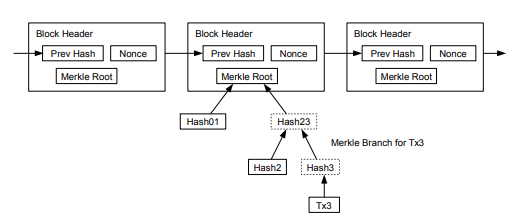
\includegraphics[scale=2.5]{img/btc.png}
			\caption{Lan't proof-of-work folosit de Bitcoin\cite{bitcoin}}
  			\label{fig:btc}
  		\end{center}
  		\end{figure} 
	
	
	
	Fiecare bloc din structura de date este identificat prin func'tia hash a header-ului blocului curent 'si a blocului anterior. Conceptul implementat de moneda virtual'a Bitcoin este urmat de alte implement'ari(Ethereum\footnote{https://www.ethereum.org/}, Hyperledger Fabric\footnote{https://hyperledger-fabric.readthedocs.io/en/latest/}, Corda\footnote{https://www.corda.net/}, etc) care au adus unele modific'ari acestei structuri, dar p'astreaza unele concepte de baz'a introduse de Bitcoin. 
	\subsection{Topologia re'telei}
	O caracteristic'a important'a a unei re'tele blockchain este lipsa unei autorit'ati centrale care s'a intermedieze tranzac'tiile din cadrul re'telei. Pentru validarea 'si propagarea tranzac'tiilor este folosit'a o re'tea peer-to-peer de participan'ti\cite{p2p}. 'In cadrul unei astfel de re'tele fiecare participant are acelea'si responsabilit'a'ti 'si privilegii, spre deosebire de o topologie client-server unde reteaua are un nod central cu capabilit'a'ti 'si responsabilit'a'ti diferite fa't'a de clien'tii din retea. Figura \ref{fig:p2p} ilustreaza diferen'ta dintre cele dou'a toplogii.
			\begin{figure}[H]
		\begin{center}
			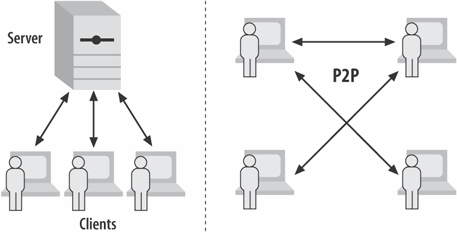
\includegraphics[scale=2]{img/p2p.png}
			\caption{Re'tea client-server vs peer-to-peer\cite{fabricdoc}}
  			\label{fig:p2p}
  		\end{center}
  		\end{figure}
Fiecare peer de'tine o copie a informa'tiilor din re'tea. Acest lucru face dificil'a modificarea abuziva a datelor, orice modificare fiind vizibil'a pentru ceilal'ti participan'ti.   
\subsection{Func'tii de hash 'si criptografie}
	O func'tie de hash reprezint'a o metoda unidirec'tional'a de mapare a unui 'sir de caractere de lungime arbitrar'a la un 'sir de caractere cu lungime fix'a. Propriet'a'tile necesare pentru o func'tie de hash sunt:
	\begin{itemize}
		\item \textbf{Calcul rapid}: efortul computa'tional pentru calcularea rezultatului trebuie sa fie mic indiferent de 'sirul de intrare.
		\item \textbf{Unidirectional'a}: ob'tinerea 'sirului original din hash nefezabil'a
		\item \textbf{Determinist'a}: rezultatul pentru un anumit 'sir de intrare este acela'si indiferent de cate ori este calculat. 
		\item \textbf{Rezistent'a la coliziuni}: oricare ar fi 'sirurile de intrare a,b func'tia de hash h(a) = h(b) doar dac'a a = b. Cu alte cuvinte un 'sir de intrare produce intotdeauna un rezultat unic.
		\item \textbf{Schimb'arile mici din 'sirul de intrare produc schimb'ari majore in rezultatul func'tiei de hash}.
\end{itemize}		
	 Printre algoritmii de hash folosi'ti de diferitele implement'ari ale tehnologiei blockchain se num'ar'a SHA256(Bitcoin)\cite{bitcoin} sau Keccak-256(Ethereum)\cite{eth-yellow}. Aceste func'tii sunt folosite 'si 'in cadrul mecanismelor  pentru stabilirea consensului.
	 
	 
		Pentru controlarea accesului in re'teaua blockchain este folosit'a metoda de criptografie cu cheie public'a. Aceasta presupune folosirea unei perechi de chei format'a dintr-o cheie privat'a 'si o cheie public'a, derivat'a din cheia privat'a. Partea public'a a cheii poate fi folosit'a pentru criptarea datelor. Datele criptate pot fi decriptate doar cu ajutorul p'ar'tii private a cheii\cite{crypto}. 
		\subsection{Mecanism de consens}
		O proprietate important'a a unei re'tele blockchain este lipsa unei autorit'a'ti centrale care sa valideze tranzac'tiile efectuate de participan'ti. Din aceast'a cauz'a apare nevoia existen'tei unor mecanisme responsabile de rezolvarea conflictelor care apar 'in cadrul re'telei 'intre 'inregistr'arile de'tinute de participan'tii din re'tea. Algorimii de consens cei mai folosi'ti sunt: Proof of Work(PoW) 'si Bizantine Fault Tolerance(BFT).
	
		PoW este algoritmul aflat in spatele unor monede virtuale precum Bitcoin 'si Ethereum. Algoritmul este conceput sub forma unei competi'tii 'in care participan'tii din re'tea 'i'si folosesc puterea de calcul pentru rezolvarea unei probleme\cite{pow}. Primul participant care rezolv'a problema prime'ste dreptul de a crea urm'atorul bloc din structura de date al'aturi de o anumit'a recompens'a. Rezolvarea problemei presupune efort masiv de calcul\cite{energy-bit} 'si din acest motiv este folosit'a drept masura de siguran'ta. Pentru a modifica intr'arile deja salvate in blockchain un atacator are nevoie de mai mult de 50\% din puterea de calcul a 'intregii retele, un astfel de atac fiind nefezabil. 'In acest mod este asigurat'a corectitudinea informa'tiilor, 'insa metoda folosit'a este ineficient'a.
		
		BFT asigur'a ajungerea la consens 'in cazul 'in care o parte din patricipan'ti sunt atacatori. Un algoritm pentru problema  cunoscut'a sub numele de "Problema generalilor bizantini"\cite{generals} a fost implementat in anul 1999 Miguel Castro and Barbara Liskov sub numele de Practical Bizantine Fault Tolerance(PBFT)\cite{pbft}. Algoritmul 'incearca ajungerea la un consens 'in cadrul sistemului, p'astr'and 'in acela'si timp o laten'ta sc'azut'a 'si eficien't'a ridicat'a. Pa'sii algoritmului sunt urm'atorii:
		\begin{itemize}
			\item Un client trimite o cerere 
			\item Cererea este transmis'a celorlal'ti clien'ti
			\item Ceilal'ti clien'ti execut'a cererea 'si transmit r'aspunsul clientului care a ini'tiat cererea
			\item Clientul a'steapt'a pan'a c'and prime'ste F + 1 r'aspunsuri identice, unde F este num'arul maxim de noduri mali'tioase tolerate
			
		\end{itemize}
		Condi'tia pentru func'tionarea corect'a a sistemului este ca num'arul de noduri mali'tioase din sistem s'a fie mai mic dec'at 1/3 din num'arul total de noduri din sistem.
		
		O compara'tie la nivel 'inalt a celor dou'a mecanisme de stabilire a consensului este prezentat'a in tabelul \ref{table1}. Tabelul prezint'a o comparatie a celor doi algoritmi lu'and 'in considerare unele propriet'a'ti importante ale unei re'tele blockchain: identitatea nodurilor, performan'ta, scalabilitatea, rezisten'ta la atacuri sau puterea consumat'a.
		
	

\begin{table}[H]
\caption{Compara'tie la nivel 'inalt: PoW vs BFT}
\centering
\begin{tabular}{|p{5cm}|p{5cm}|p{5cm}|}      
\hline\hline                        
 & Proof of Work & Bizantine Fault Tolerance \\ [0.5ex]  
\hline                             
Managementul identit'a'tii nodurilor & deschis, decentralizat & fiecare nod trebuie s'a cunoasc'a inform'atii despre celelalte noduri\\ 
\hline  
Scalabilitate & excelent'a & limitat'a \\              
\hline 
Performan'ta(throuput) & limitat'a & excelent'a(mii de tranzac'tii/sec	\\
\hline 
Performan'ta(laten'ta) & laten'ta crescut'a & excelent'a(similar'a cu cea indusa de re'tea) \\
\hline 
Putere consumat'a & Ridicat'a(PoW necesit'a putere de calcul ridicat'a) & Scazut'a \\
\hline 
Num'ar total de atacatori tolera'ti & 25\% din puterea de calcul  & 33\% din num'arul de noduri care voteaz'a\\[1ex]
           
\hline                              
\end{tabular}
\label{table1} 
\end{table}

Se poate observa faptul ca algoritmii reprezint'a dou'a abord'ari diferite in cadrul unei re'tele blockchain. PoW pune accent pe scalabilitate dar prezint'a o performan't'a sc'azut'a 'in timp ce BFT asigur'a performan'ta ridicat'a dar cu o scalabilitate redus'a. Decizia 'in ce prive'ste tipul de algoritm folosit depinde de nevoia sistemelor implementate.
	\subsection{Smart contract}
	Un smart contract reprezint'a "un set de promisiuni 'in format digital in care p'artile implicate ac'tioneaz'a conform acestor promisiuni"\cite{sc}. Altfel spus aceste contracte sunt o reprezentare digital'a a unor clauze contractuale, integrate in software pentru a media ac'tiuni prin opera'tii bazate pe reguli. Odat'a ce precondi'tiile pentru un smart contract sunt indeplinite 'si acesta este ini'tiat ac'tiunile din cadrul lui sunt executate, ele fiind irevocabile.
	\subsection{Implement'ari ale tehnologiei blockchain}
	Prima implementare cu succes a tehnologiei blockchain a fost realizat'a de moneda virtual'a bitcoin. Odat'a cu cre'sterea acesteia in popularitate au ap'arut diverse implement'ari ale acestei tehnologii, fiecare av\^and unele particularit'a'ti 'si scopuri de utilizare diferite.
	
	
	\textbf{Tipuri de implement'ari}. Exist'a 3 tipuri de implement'ari ale tehnologiei blockchain: public, privat si bazat pe permisiuni\cite{permiss}\cite{ppp}. Tabelul \ref{table2} prezint'a o analiz'a la nivel 'inalt a celor 3 tipuri de implement'ari. Sunt luate 'in considerare aspecte precum drepturile de acces, performan'ta, costurile implicate, avantajele 'si dezavantajele fiecarei implement'ari precum 'si num'arul de puncte de e'sec 'in cazul fiec'areia.
		
	\textbf{Blockchain public}. In cadrul unul blockchain public nu exist'a nevoia definirii unor  drepturi de acces. Orice entitate are drepturi de acces egale 'in cadrul re'telei 'si poate participa la procesul de validare a tranzac'tiilor. Din acest punct de vedere un blockchain public folose'ste o topologie decentralizat'a nefiind prezent'a o autoritate centrala care s'a medieze tranzac'tiile din re'tea. O astfel de implementare este folosit'a de catre monedele virtuale Bitcoin sau Ethereum. 'In cadrul acestor re'tele participan'tii efectuaz'a tranzac'tii f'ar'a a fi implicat'a o a treia entitate 'in acest proces. Pentru a se ajunge la un consens, un mecanism de tip PoW este folosit, acesta av'and un impact asupra performan'tei re'telei 'si a consumului de enegie 'si resurse\cite{energy-bit}.
	
	\textbf{Blockchain privat}. Spre deosebire de un blockchain public, cel privat folose'ste o topologie centralizat'a. Accesul la re'tea este controlat de o autoritate central'a, aceasta av\^and dreptul de a lua decizii 'si de a implementa reguli 'in cadrul re'telei. Un astfel de blockchain poate fi folosit in cazul in care este necesara restric'tionarea accesului publicului larg la re'tea. O astfel de re'tea se bazaz'a pe stabilirea unui nivel ridicat de 'incredere 'in autoritatea central'a responsabil'a de administrarea re'telei. Deoarece doar o singura entitate este responsabil'a de procesul de validare a tranzac'tiilor, apare avantajul performan'tei crescute 'in compara'tie cu un blockchain public.
	
	\textbf{Blockchain bazat pe permisiuni}. Acesta abordare poate fi v'azut'a ca un hibrid 'intre un blockchain privat 'si unul public. Autoritatea 'in re'tea este de'tinut'a de un set de entit'a'ti care pot face parte din organiza'tii diferite. Aceste entit'a'ti stabilesc drepturile de acces la re'tea 'si particip'a la validarea tranzac'tiilor. Drepturile de acces depind de identit'a'tile participan'tilor, fiind nevoie de executarea unor smart contracts 'inainte de executarea unor tranzac'tii pentru validarea identit'a'tii participan'tilor. Hyperledger Fabric\cite{hlfv} si Corda sunt implement'ari ale unui astfel de blockchain. Ambele sunt solu'tii open-source care pot fi folosite pentru stocarea si partajarea datelor 'intre participan'tii retelei. Ambele ofera solu'tii pentru implementarea unei retele distribuite pentru stocarea inregistrarilor, pun\^an\^ad accent pe protejarea datelor 'si siguran'ta acestora.
	
	
\begin{table}[h]
\caption{Compara'tie la nivel 'inalt a implement'arilor tehnologiei blockchain}
\label{table2}
\resizebox{\textwidth}{!}{%
\begin{tabular}{|l|l|l|l|}
\hline
                                                          & Public                                                                                                                                                                                                             & Privat                                                                                                                                                                                    & Bazat pe permisiuni                                                                                                                                                                                                                                                   \\ \hline
Topologie re'tea                                           & decentralizat'a                                                                                                                                                                                                     & \begin{tabular}[c]{@{}l@{}}partial\\ decentralizat'a\end{tabular}                                                                                                                          & \begin{tabular}[c]{@{}l@{}}partial\\ decentralizat'a\end{tabular}                                                                                                                                                                                                      \\ \hline
Definire                                                  & \begin{tabular}[c]{@{}l@{}}Oricine are acces \\ la datele din re'tea. \\ Toate nodurile \\ particip'a la validare\end{tabular}                                                                                       & \begin{tabular}[c]{@{}l@{}}Permisiunile de acces \\ sunt controlate de o \\ singur'a entitate de \\ 'incredere din re'tea\end{tabular}                                                       & \begin{tabular}[c]{@{}l@{}}Permisiunile de acces\\ sunt controlate de un \\ num'ar prestabilit \\ de noduri cu autoritate\end{tabular}                                                                                                                                 \\ \hline
Beneficii                                                 & \begin{tabular}[c]{@{}l@{}}- Sigur, deoarece to'ti \\ participan'tii contribuie \\ la validarea tranzac'tiilor\\ - Transparent, toate \\ tranzac'tiile fiind publice\\ iar entit'a'tile implicate\\ anonime\end{tabular} & \begin{tabular}[c]{@{}l@{}}- Verificare eficient'a \\ a tranzac'tiilor de c'atre\\ autoritatea central'a\\ - Autoritatea central'a \\ decide entita'tile care \\ au acces la re'tea\end{tabular} & \begin{tabular}[c]{@{}l@{}}- Eficient, deoarece un\\ num'ar relativ mic de\\ noduri verific'a tranzac'tiile\\ - Drepturile de acces sunt \\ controlate de un set \\ predeterminat de noduri\\ - Controlul nu este de'tinut \\ de c'atre o autoritate central'a\end{tabular} \\ \hline
Provoc'ari                                                 & Eficien'ta sc'azut'a                                                                                                                                                                                                  & \begin{tabular}[c]{@{}l@{}}Controlul este de'tinut\\ de o singur'a entitate\end{tabular}                                                                                                    &                                                                                                                                                                                                                                                                       \\ \hline
Cost                                                      & sc'azut                                                                                                                                                                                                             & ridicat                                                                                                                                                                                   & mediu                                                                                                                                                                                                                                                                 \\ \hline
Performan'ta                                               & sc'azut'a                                                                                                                                                                                                            & excelent'a                                                                                                                                                                                 & ridicat'a                                                                                                                                                                                                                                                              \\ \hline
\begin{tabular}[c]{@{}l@{}}Puncte de \\ e'sec\end{tabular} & n                                                                                                                                                                                                                  & 1                                                                                                                                                                                         & * (nodurile cu autoritate)                                                                                                                                                                                                                                            \\ \hline
\end{tabular}%
}
\end{table}

Se observ'a c'a eficien'ta 'si performan'ta re'telei scad odat'a cu cre'sterea decetraliz'arii acesteia. Aceasta se datoreaz'a metodei de stabilire a consensului 'si a num'arului de entit'a'ti implicate in acest mecanism.
	
\subsection{Ethereum, Hyperledger Fabric, Corda}
'In continuare sunt este prezentat'a o compara'tie 'intre principalele solu'tii disponibile pentru implementarea unei re'tele distribuite folosind tehnologia blockchain. Aceste solu'tii sunt: Ethereum, Hyperledger Fabric si Corda\cite{comp}. Tabelul \ref{table4} prezint'a o comparatie a caracteriticilor celor 3 solu'tii:



\begin{table}[H]
\caption{Comparatie Ethereum, Hyperledger Fabric, Corda conform cu\cite{comp}}
\centering
\begin{tabular}{|p{3cm}|p{3cm}|p{3cm}|p{3cm}|}      
\hline\hline                        
Caracteristica  & Ethereum & Hyperledger Fabric & Corda \\ [0.5ex]  
\hline                             
descriere & platforma generic'a blockchain & platform'a modular'a blockchain & solu'tie distribuit'a pentru domeniul financiar\\ 
\hline  
mod de operare  & f'ar'a permisiuni, public, privat & bazat pe permisiuni, privat & bazat pe permisiuni, privat\\              
\hline 
consens & PoW & suport pentru diferite mecanisme & consens realizat de "notary nodes" \\
\hline 
smart contract  & Solidity& Go, Java& Kotlin, Java \\
\hline 
moneda virtual'a & Ether & f'ar'a,  poate fi implementat'a cu ajutorul smart contract& f'ar'a  \\[1ex]
           
\hline                              
\end{tabular}
\label{table4} 
\end{table}

Ethereum si Hyperledger Fabric sunt g\^andite pentru utilizarea 'intr-un spectru larg de cazuri de utilizare. Spre deosebire de acestea, Corda are ca utilizare principal'a domeniul financiar\cite{cordadoc}.

'In ce prive'ste mecansimul de consens Hyperledger Fabric ofer'a posibilitatea utiliz'arii a diferite mecansime de consens. Stabilirea consensului are loc la  nivelul tranzac'tiilor 'si implic'a doar par'tile care sunt responsabile de  tranzac'tie. Nodurile din re'tea de'tin roluri diferite 'in ob'tinerea consensului. Hyperledger Fabric 'imparte nodurile din sistem 'in 3 categorii: \emph{peer, orderer, client}\cite{fabricdoc}\cite{hlfv}. Nodurile de tip \emph{peer} mentin registrul cu date si primesc mesaje pentru actualizarea registrului. Nodurile de tip \emph{client} reprezinta utilizatorii retelei si au capabilitatea de a invoca tranzactii. Comunicarea intre \emph{peer}-uri prin intermediul canalelor de comunicare este asigurata de nodurile de tip \emph{orderer}.

Corda foloseste o abordare similara cu Hyperledger Fabric pentru stabilirea consensului. Aceasta are loc la nivelul tranzactiilor si utilizeaza doar partile implicate. Consensul trebuie determinat intre participantii retelei numiti \emph{notary nodes}\cite{cordadoc}, existand libertatea alegerii algoritmului folosit.

Spre deosebire de cele doua abord'ari de mai sus, Ethereum folose'ste un mecanism PoW. Acest aspect duce la sc'aderea performan'tei procesarii tranzac'tiilor. 

Lucarea folose'ste 'in continuare platforma Hyperledger Fabric pentru implementarea sistemului. Principala motive pentru utilizarea acestei platforme sunt flexibilitatea oferit'a 'in implementarea cazurilor de utilizare. Spre deosebire de Corda, cu specializare pe domeniul financiar, Hyperledger Fabric 'si Ethereum pot fi aplicate 'intr-un spectu larg de domenii. Performan'ta este un alt motiv pentru alegerea platformei Hyperledger Fabric. Posibilitatea de alegere a mecanismului de consens, spre deosebire de Ethereum, duce la imbun'at'a'tirea performan'tei 'in ce prive'ste timpul de procesare a tranzac'tiilor. 

\section{Scenarii de utilizare ale tehnologiei blockchain}
Sec'tiunea curenta descrie unele scenarii de utiliare 'in anumite domenii care pot beneficia de pe urma utiliz'arii tehnologiei blockchain. Sunt prezentate aspecte ale tehnologiei blockchain care pot ajuta la imbun'at'a'tirea metodologiilor din aceste domenii.

\textbf{Determinarea identit'a'tii digitale}. 'In prezent, detaliile despre identitatea unei persoane sunt stocate de c'atre diferite institu'tii. Din acest motiv o persoana poate avea o serie de identit'a'ti asupra carora nu de'tine controlul. Apar provoc'ari 'in ce prive'ste siguran'ta datelor cu caracter personal 'si a existen'tei unui punct unic de e'sec. 

Tehnologia blockchain poate imbun'at'a'tii procedurile din acest domeniu. Prin oferirea controlului absolut asupra identit'a'tii lor, participan'tii pot alege detaliile care vor s'a le partajeze despre identitatea lor. Aceasta identitate a unui utilizator nu va fi stocat'a de o alta entitate, ci aceste etit'a'ti vor contribui doar la validarea detaliilor despre identitatea unei persoane.

\textbf{Managementul datelor financiare}. Domeniul finaciar este predispus fraudelor deoarece sistemele de contabilitate sunt controlate de entit'a'tile care le folosesc. Este necesar, de asemenea un efort uman considerabil pentru medierea tranzac'tiilor 'intre sisteme incompatibile. Toate acestea determin'a costuri ridicate de mentenan'ta, efort uman 'si timp.

Utilizarea smart contracts 'in domeniul financiar poate imbun'at'a'tii timpul de procesare a tranzac'tiilor, corectitudinea datelor 'si transparen'ta acestora. Este eliminat'a nevoia existen'tei entitatilor care sa medieze tranzac'tiile 'intre anumite p'arti, acestea av\^and posibilitatea de a tranzac'tiona 'in mod direct. Fraudarea datelor este mai dificil'a, sistemul de contabilitate fiind controlat de toate entit'a'tile implicate. 

\textbf{Determinarea provenien'tei bunurilor}. Determinarea originii anumitor bunuri 'intr-un lan't de aprovizionare 'intampin'a dificult'a'ti din cauza complexit'a'tii procesului de management al unui lan't de aprovizionare 'si dorin'tei de a partaja informa'tii doar cu entit'a'tile relevante(institu'tii de reglementare, vamale, etc). Din cauza dificult'a'tilor 'int\^alnite 'in determinare originii produselor riscul existen'tei fraudelor este ridicat.

Urm'arirea provenien'tei produselor poate fi imbun'at'a'tit'a prin folosirea unei re'tele blockchain pentru 'inregistrarea datelor referitoare la originea produselor. Accesul la informa'tii este simplificat, entit'a'tile din re'tea participand la validarea si memorarea tranzac'tiilor 'in registrul de date comun. Detectarea fraudelor este imbun'at'a'tita, fiecare entitate av\^and acces la tranzac'tiile din sistem. 

\section{Tehnologia blockchain 'in studiile clinice}
Principalele provoc'ari 'intampinate 'in cadrul studiilor clinice sunt legate de protec'tia datelor cu caracter personal 'si reducerea num'arului de fraude din acest domeniu.

Tehnologia blockchain poate avea un impact global asupra cercet'arii clinice deoarece permite urm'arirea, partajarea 'si protec'tia informa'tiilor. Prin utilizarea unui sistem decentralizat folosit pentru urm'arirea activit'a'tilor din cadrul unui studiu clinic 'si a unei re'tele peer-to-peer pentru partajarea informa'tiilor sunt asigurate transparen'ta 'si protec'tia datelor personale ale pacientilor. Un sistem bazat pe aceasta tehnologie poate imbun'at'a'ti metodologiile din cercetarea clinic'a 'si protectia datelor cu caracter sensibil.

\subsection{Modelarea cercet'arii clinice sub forma unei re'tele de\\ afaceri}

	O \textbf{retea de afaceri} reprezint'a o re'tea complex'a de companii "unde scopul este de a sus'tine cerin'tele informa'tionale 'si opera'tionale ale afacerii cum ar fi cele de marketing, contabilitate ..."\cite{bndef}. Un alt aspect important al unei re'tele de afaceri este c'a aceasta nu 'inglobeaza doar afacerea 'in sine ci implic'a 'si unele entit'a'ti din exterior care sus'tin activitatea re'telei cum ar fi furnizorii sau distribuitorii. 
	
	'In cazul studiilor clinice o re'tea de afaceri poate fi format'a din participan'tii direc'ti la activita'ti(ex. centrele medicale 'in care se desfasoar'a studiile clinice), precum 'si par'tile care sus'tin activitatea studiilor clinice(ex. furnizori, institu'tii de reglementare...)
	Re'telele existente de afaceri folosesc 'in prezent metode similare pentru stocarea informa'tiilor. Entit'atile implicate tranzac'tioneaz'a 'intre ele, 'ins'a men'tin 'inregistr'ari proprii referitoare la tranzac'tiile efectuate. 'In cele mai multe cazuri o autoritate central'a 'in care toate partile implicate au incredere intermediaz'a tranzactiile 'si schimbul de informa'tii din cadrul re'telei. Conceptul descris mai sus este ilustrat in figura \ref{fig:centralised}.\\	
		\begin{figure}[H]
		\begin{center}
			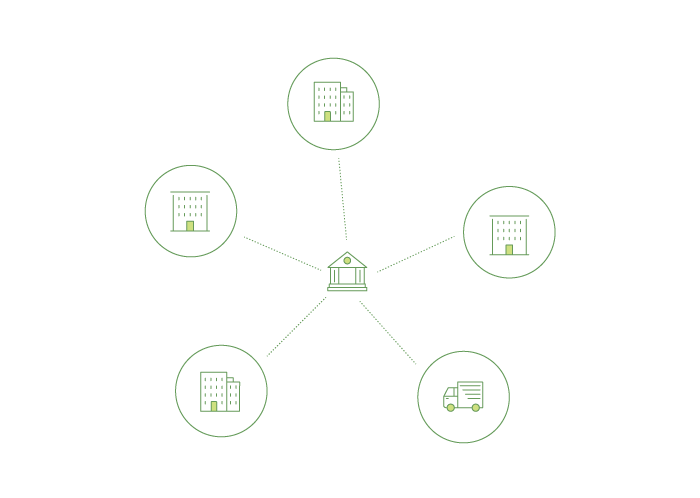
\includegraphics[scale=1.60]{img/current_network.png}
			\caption{Re'tele de afaceri centralizate\cite{fabricdoc}}
  			\label{fig:centralised}
  		\end{center}
  		\end{figure}
  		
	Aceasta metod'a prezint'a o complexitate redus'a dar produce 'in acela'si timp unele dezavantaje. Partajarea informa'tiilor este efectuat'a indirect, responsabil'a de acest lucru fiind autoritatea central'a. Din acest motiv procesul este 'incetinit, implic'and costuri suplimentare. Stabilirea corectitudinii informa'tiilor devine dificil'a 'in momentul 'in care par'tile implicate de'tin inregistrari diferite referitoare la tranzactii.
		Printre sistemele care folosesc o astfel de abordare se numar'a Oracle Siebel Clinical Trial Management System\cite{ctms}. Sistemul ofer'a posibilitatea cercet'atorilor de a organiza 'si colecta date 'in cadrul unui studiu clinic, fiind astfel simplificat'a activitatea acestora. Datele sunt colectate intr-o baza de date central'a . Partajarea datelor 'intre participan'ti are loc fie prin implicarea unei autorit'a'ti centrale, fie prin folosirea unor mijloace nesigure. Aceste mijloace sunt ineficiente 'si reprezint'a un risc 'in ce prive'ste protejarea datelor cu caracter sensibil.\\	

\textbf{Re'tele de afaceri decentralizate}. O alt'a abordare pentru realizarea unei re'tele de afaceri reprezint'a utilizarea unei re'tele decentralizate. O astfel de metod'a presupune folosirea unui registru comun, replicat de catre fiecare participant din re'teaua de afaceri. Procesul de salvare a tranzac'tiilor 'in cadrul registrului este de asemenea partajat, fiecare participant la re'tea contribuind la procesul de validare 'si memorare a tranzac'tiilor efectuate. Este eliminat'a astfel nevoia unei autorit'a'ti centrale, par'tile implicate av'and 'incredere ca tranzac'tiile salvate 'in registrul comun sunt valide. \\
Figura \ref{fig:decentralised} ilustreaza structura unei re'tele de afaceri decentralizate. O astfel de re'tea este similar'a cu o re'tea blockchain.
		\begin{figure}[H]
		\begin{center}
			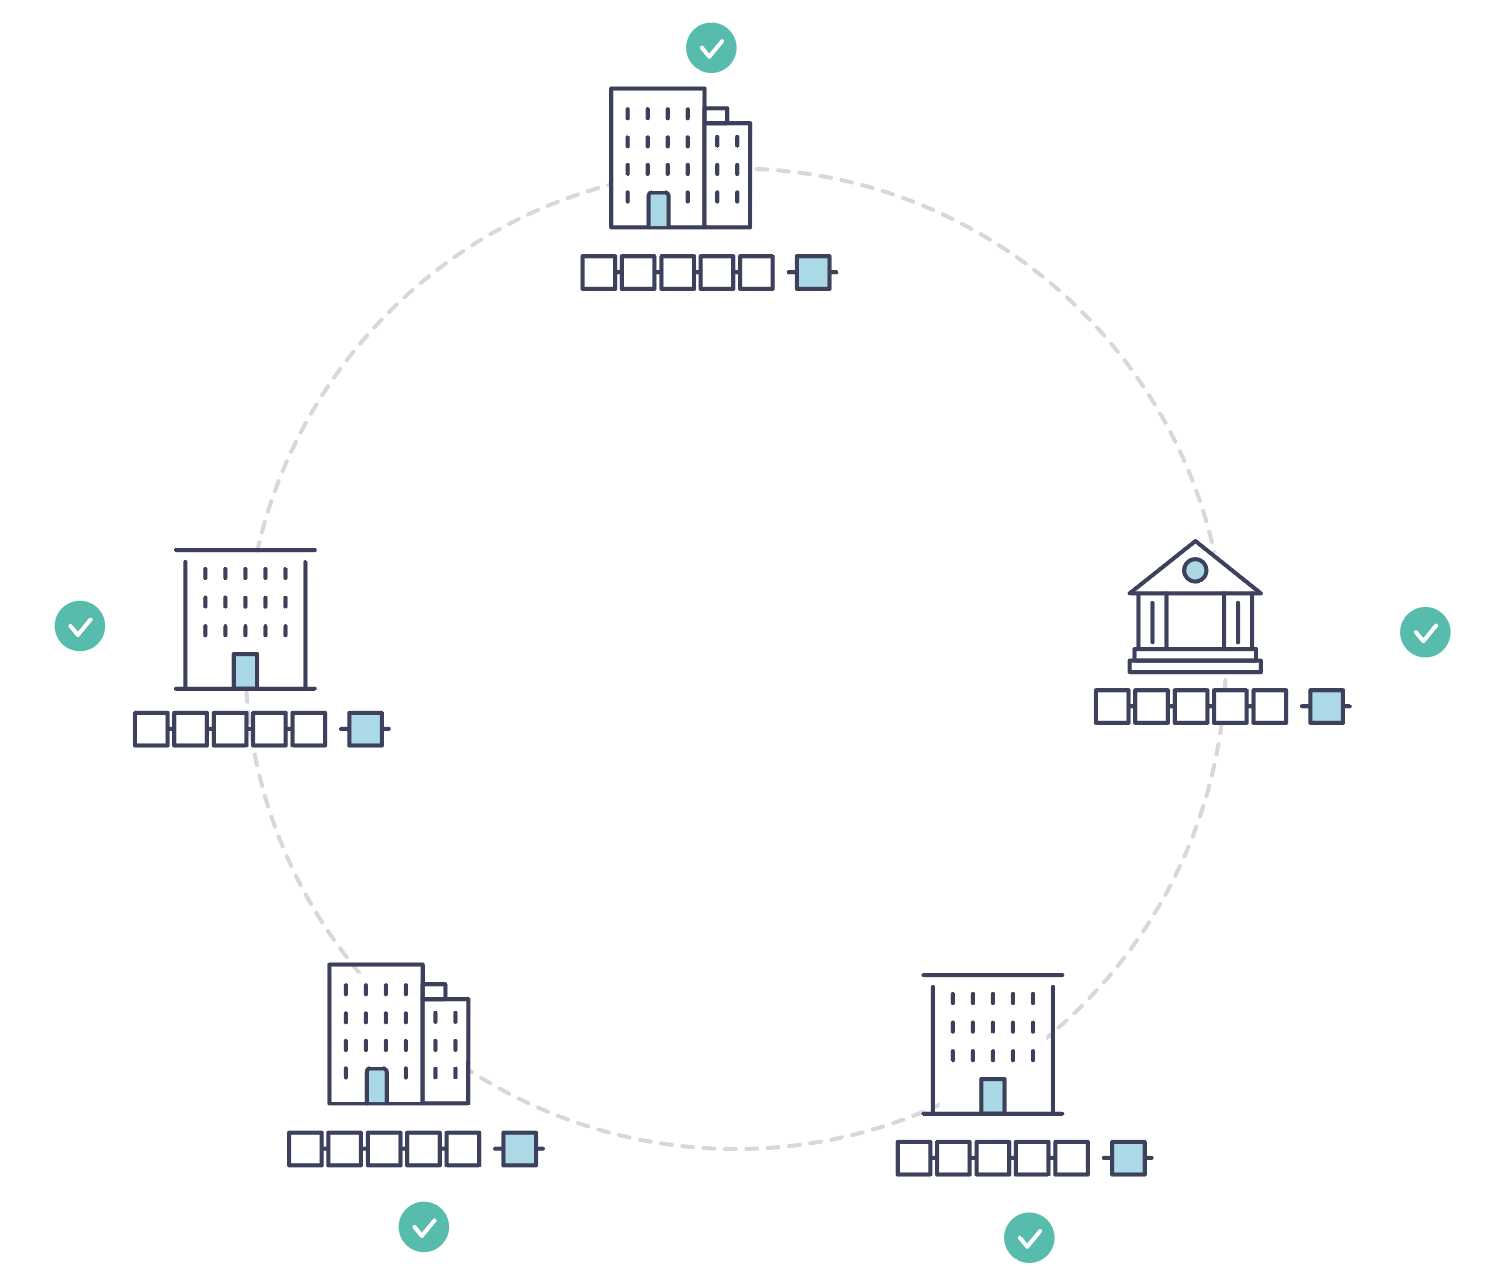
\includegraphics[scale=0.3]{img/future_net.png}
			\caption{Re'tele de afaceri decentralizate\cite{fabricdoc}}
  			\label{fig:decentralised}
  		\end{center}
  		\end{figure}
  		

\chapter{Analiz'a 'si Fundamentare Teoretic'a}
\label{ch:analysis}
Acest capitol prezint'a cerin'tele unui sistem pentru managementul studiilor clinice. Sunt prezenta'ti actorii principali ai sistemului, al'aturi de cazurile de utilizare asociate fiec'aruia. Capitolul se 'incheie printr-o prezentare a tehnologiilor folosite pentru implementarea cazurilor de utilizare, respect\^and constr\^angerile specificate de cerin'tele sistemului.

\section{Cerin'te sistem}
Sec'tiunea prezint'a o analiz'a a sistemului pentru managementul studiilor clinice. Cerin'tele unui sistem pot fi clasificate 'in cerin'te func'tionale 'si non-func'tionale. Cerin'tele func'tionale descriu comportamentul sistemului din punctul de vedere al utilizatorilor. Cerin'tele non-func'tionale descriu propriet'a'ti 'si impun constr\^angeri asupra sistemului.

\subsection{Cerinte func'tionale}
'In continuare sunt prezentate cerin'tele func'tionale 'indeplinite de modulul client al aplica'tiei. Aceste functionalit'a'ti sunt disponibile pentru utilizatorii sistemului:
\begin{enumerate}
	\item \textbf{Autentificare}: Accesul la func'tionalit'a'tile aplica'tiei este disponibil doar pentru utilizatorii autentifica'ti. Identitatea utilizatorului are o importan't'a major'a in cadrul retelei blockchain. 'In acest mod este asigurat'a posibilitatea  urm'ariri activitatii participantilor 'si salvarea unui istoric a tuturor opera'tiilor efectuate de ace'stia. 
	\item \textbf{Management identitate}: Utilizatorii autentifica'ti au nevoie de o identitate emisa de organiza'tia din care fac parte pentru a putea accesa reteaua. Cu ajutorul acesteia utilizatorii sunt identifica'ti 'in re'teaua blockchain 'si supu'si regulilor de acces la resurse definite 'in sistem. Identitatea unui participant poate fi revocat'a, acesta pierz\^and accesul la serviciile oferite de sistem.
	\item \textbf{Management studii clinice}: Utilizatorii au posibilitatea de a crea un nou studiu clinic folosind interfa'ta utilizator dup'a introducerea informa'tiilor necesare.  Utilizatorii autentifica'ti care au drepturile de acces necesare pot accesa informa'tiile despre un studiu clinic 'si datele legate de activitatea desf'a'surat'a 'in cadrul acestora.
	\item \textbf{'Inrolare pacien'ti}: Posibilitatea de a asocia un pacient la un studiu clinic.
	\item \textbf{Colectare date}: Cercet'atorii pot defini 'in cadrul unui studiu clinic formulare de colectare a datelor de la pacien'ti. Aceste formulare ofer'a cercet'atorului flexibilitatea de a defini c'ampuri de text 'si 'intrebari cu variante de r'aspuns relevante pentru studiul clinic. Folosind formularele definite, cercet'atorii au posibilitatea de a colecta date de la un anumit pacient.
	\item \textbf{Drepturi de acces}: Permite administratorilor sistemului s'a defineasc'a drepturile de acces la resursele 'si serviciile oferite de aplica'tie.
	\item \textbf{Gestionare fi'siere}: Utilizatorii care de'tin drepturile necesare pot salva 'in sistem fi'siere de protocol 'si contracte de sponsorizare. Protocolul unui studiu clinic descrie modul de desf'a'surare al acestuia. Utilizatorii care de'tin drepturile de acces necesare pot 'inc'arca un fi'sier de protocol 'si 'il pot desc'arca prin intermediul interfe'tei utilizator.
	\item \textbf{Istoric activit'a'ti}: Sistemul colecteaz'a 'in mod automat un istoric in timp al opera'tiilor efectuate de utilizatori. 
\end{enumerate}

\subsection{Cerinte non-func'tionale}
\begin{enumerate}
\item \textbf{Utilizabilitatea}. Procesele din cadrul unui studiu clinic au o complexitate ridicat'a. Din acest motiv sistemul are nevoie de o interfa't'a utilizator intuitiv'a, care s'a permit'a cercetatorilor s'a 'i'si desf'a'soare activitatea rapid. Un alt aspect important este correctitudinea informa'tiilor care poate fi imbun'at'a'tit'a prin valid'ari 'si mesaje de eroare.
\item \textbf{Securitatea}. Protec'tia datelor cu caracter sensibil are o importan't'a majora 'in studiile clinice. Accesul pentru citirea 'si scrierea datelor este oferit doar utilizatorilor autentifica'ti. 'In plus, accesul la resurse este controlat de listele de acces care definesc reguli de scriere s'i citire.
\item \textbf{Fiablitate}. Timpul i'n care serviciile oferite de sistem sunt indisponibile trebuie s'a fie minim. Acest lucru poate fi asigurat prin replicarea nodurilor din re'teaua blockchain.
\item \textbf{Performan'ta}. Performan'ta sistemului este masurat'a folosind mijloace specifice tehnologiei utilizate. Aceasa poate fi m'asurat'a 'in num'arul de tranzac'tii/secund'a sau resursele de sistem consumate.
\item \textbf{Compatibilitate}. Cerin'ta non-func'tional'a care specific'a posibilitatea de utilizare a sistemului din platforme multiple. 'In cazul sistemului de management a studiilor clinice este posibil accesul utilizatorilor din orice browser modern, mobil sau desktop. 
\end{enumerate}

\section{Cazuri de utilizare}
Sec'tiunea descrie cazurile de utilizare ale aplica'tiei analiz'and actorii implica'ti 'in realizarea acestora. Sistemul pentru managementul studiilor clinice are definite 4 tipuri principale de utilizatori: administrator, cercet'ator, agent de reglementare 'si sponsor.
\begin{table}[H]
\centering
\caption{Asociere func'tionalit'a'ti - cazuri de utilizare - actori}
\label{uc-table}
\begin{tabular}{|p{5cm}|p{5.3cm}|p{5.1cm}|}
\hline
\hline
Func'tionalitate          & Cazuri de utilizare                        & Actori                                                 \\ \hline
Autentificare            & Autentificare utilizator                   & Cercet'ator, Agent Reglementare, Sponsor, Administrator \\ \cline{2-3} 
                         & Mapare identitate la contul utilizatorului & Cercet'ator, Agent Reglementare, Sponsor                \\ \hline
Management identitate    & Emitere identitate                         & Administrator                                          \\ \cline{2-3} 
                         & Revocare identitate                        & Administrator                                          \\ \hline
Management studiu clinic & Creare studiu clinic                       & Cercet'ator                                             \\ \cline{2-3} 
                         & Vizualizare studiu clinic                  & Cercet'ator, Agent Reglementare, Sponsor                \\ \cline{2-3} 
                         & C'autare studii clinice                     & Cercet'ator, Agent Reglementare, Sponsor                \\ \cline{2-3} 
                         & Modificare studiu clinic                   & Cercet'ator                                             \\ \hline
'Inrolare pacien'ti        & Creare pacient                             & Cercet'ator, Administrator                              \\ \cline{2-3} 
                         & C'autare pacient                            & Cercet'ator, Administrator                              \\ \cline{2-3} 
                         & 'Inrolare pacient 'in studiu clinic          & Cercetator                                             \\ \hline
Colectare date           & Creare formular personalizat               & Cercet'ator                                             \\ \cline{2-3} 
                         & Vizualizare formulare                      & Cercet'ator, Agent Reglementare                         \\ \cline{2-3} 
                         & Completare formular                        & Cercet'ator                                             \\ \cline{2-3} 
                         & Vizualizare date colectate                 & Cercet'ator, Agent Reglementare, Sponsor                \\ \hline
Drepturi de acces        & Asignare cercet'ator la studiu clinic       & Cercet'ator                                             \\ \cline{2-3} 
                         & Asignare agent reglementare                & Administrator                                          \\ \hline
Gestionare fi'siere       & Ad'augare fi'sier                            & Cercet'ator, Sponsor                                    \\ \cline{2-3} 
                         & Desc'arcare fi'sier                          & Cercet'ator, Sponsor                                    \\ \hline
Istoric activit'a'ti       & Creare istoric                             & Sistem                                                 \\ \cline{2-3} 
                         & Vizualizare istoric                        & Cercet'ator, Agent Reglementare, Sponsor                \\ \cline{2-3} 
                         & Filtrare istoric                           & Cercet'ator, Agent Reglementare, Sponsor                \\ \hline
\end{tabular}
\end{table}

 Aceste 3 tipuri de utilizatori apar'tin unor organiza'tii diferite din re'teaua blockchain. Tabelul \ref{uc-table} prezint'a o asociere 'inte functionalit'a'tile sistemului, cazurile de utilizare s'i utilizatorii care particip'a la realizarea acestora.


\subsection{Cercetator} Utilizatorul apar'tine organiza'tiilor din domeniul medical 'in cadrul re'telei blockchain. Responsabilitatea sa principal'a este managementul activit'a'tilor din cadrul unui studiu clinic. 'In figura \ref{fig:ucc} sunt prezentate cazurile de utilizare asociate utilizatorului.

	\begin{figure}[H]
		\begin{center}
			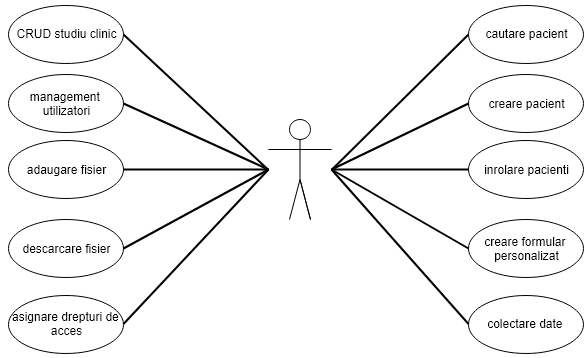
\includegraphics[scale=0.6]{img/uc_cerc.PNG}
			\caption{Cazuri de utilizare cercetator}
  			\label{fig:ucc}
  		\end{center}
  	\end{figure}
  		
 
 

\subsection{Agent de reglementare} Utilizatorul apar'tine intitu'tiilor care se ocup'a de aplicarea regulilor asupra unui studiu clinic. Aces'tia supervizeaz'a acivit'a'tile care au loc 'in cadrul unui studiu clinic cu scopul de a g'asi eventualele nereguli. Figura \ref{fig:ucr} prezint'a cazurile de utilizare 'si responsabilit'a'tile asociate agentului de reglementare.

	\begin{figure}[H]
		\begin{center}
			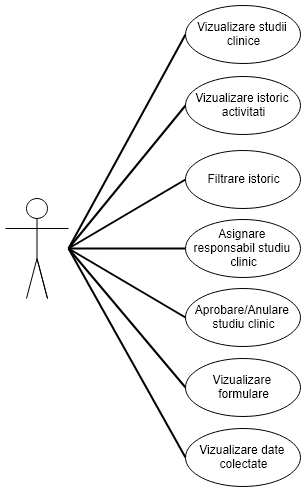
\includegraphics[scale=0.5]{img/uc_reg.PNG}
			\caption{Cazuri de utilizare agent de reglementare}
  			\label{fig:ucr}
  		\end{center}
  	\end{figure}

\subsection{Sponsor} 
    Interesat de rezultatele studiilor clinice finan'tate. Dore'ste sa poat'a vizualiza rezultatele ob'tinute 'in timpul unui studiu clinic. Particip'a la 'incheierea contractelor de sponsorizare cu institu'tiile responsabile de organizarea studiilor clinice. 'In figura \ref{fig:ucs} sunt reprezentate cazurile de utilizare asociate utilizatorului de tip sponsor.

	\begin{figure}[H]
		\begin{center}
			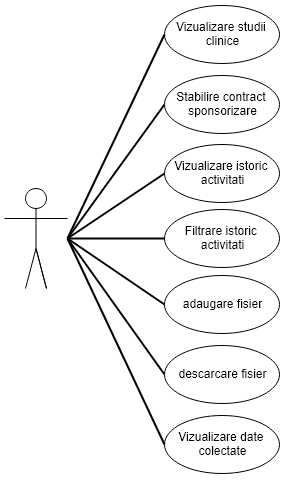
\includegraphics[scale=0.5]{img/uc_spon.PNG}
			\caption{Cazuri de utilizare sponsor}
  			\label{fig:ucs}
  		\end{center}
  	\end{figure}


\subsection{Descrierea cazurilor de utilizare}
  		
 \subsubsection{Caz de utilizare 1 - Autentificare}
 Este prezentat'a 'in continuare o descriere a mecanismului de autentificare a utilizatorilor in sistem. Aceasta descriere con'tine scenariul principal de succes al'aturi de extensiile cazului de utilizare\\
\textbf{Numele cazului de utilizare:} Autentificare utilizator\\
\textbf{Actor principal:} Utilizator al sistemului\\
\textbf{Stakeholders:}
\begin{itemize}
    \item Utilizatorul: dore'ste sa acceseze serviciile oferite de sistem
    \item Administrator: dore'ste ca doar utilizatorii cu identit'a'ti emise sa poata accesa sistemul
\end{itemize}
\textbf{Precondi'tii:} f'ar'a\\
\textbf{Postcondi'tii:} sistemul determin'a identitatea utilizatorului, o afi'seaza si ofera acces la serviciile sistemului\\
\textbf{Scenariu de succes:} 
\begin{enumerate}
     \item Utilizatorul selecteaz'a op'tiunea de autentificare
     \item Aplica'tia redirec'tioneaz'a utilizatorul spre sistemul extern de autentificare
     \item Utilizatorul introduce creden'tialele de acces
     \item Sistemul extern furnizeaz'a un token de autentificare
     \item  Aplica'tia afi'seaz'a identitatea utilizatorului 'si ii permite accesul
\end{enumerate}
\textbf{Scenarii alternative:}
\begin{itemize}
    \item 3a. Utilizatorul introduce creden'tiale gre'site:
        \begin{enumerate}
            \item Sistemul extern afi'seaza un mesaj de eroare 'si solicita creden'tialele
        \end{enumerate}
    \item 3b. Utilizatorul este la prima autentificare 'in sistem
        \begin{enumerate}
            \item Sistemul extern cere permisiunea pentru autorizarea aplica'tiei
            \item Utilizatorul selecteaza optiune de autorizare acces
            \item Sistemul extern furnizeaza un token de autentificare
        \end{enumerate}
    \item 5a. Utilizatorul nu are o identitate definit'a 'in re'tea
        \begin{enumerate}
            \item Aplica'tia cere un cod de inrolare i'n sistem
            \item Utilizatorul introduce codul furnizat de administra'tia organiza'tiei din care face parte
            \item Aplica'tia salveaza o asociere 'intre identitatea utilizatorului 'si contul acestuia
        \end{enumerate}
\end{itemize}

\subsubsection{Caz de utilizare 2 - Creare formular personalizat}
Cercet'atorii au la dispozitie o func'tionalitate prin care pot defini un formular 'in func'tie de nevoile 'int\^alnite 'in cadrul unui studiu clinic. 'In continuare sunt descri'si actorii implica'ti, al'aturi de pa'sii care trebuie urma'ti 'in definirea unui formular.
\textbf{Numele cazului de utilizare:} Creare formular personalizat\\
\textbf{Actor principal:} Cercet'ator\\
\textbf{Stakeholders:}
\begin{itemize}
    \item Cercet'ator: doreste ca sistemul s'a ii ofere flexibilitatea de a defini c\^ampurile de care are nevoie intr-un formular
    \item Agent de reglementare: interesat de corectitudinea datelor colectate. Dore'ste sa aib'a acces la informa'tii
    \item Sponsor: interesat de structura formularului de colectare a datelor
\end{itemize}
\textbf{Precondi'tii:} Utilizator autentificat, cu drepturi de citire 'si scriere asupra unui studiu clinic\\
\textbf{Postconditii:} Formularul definit este salvat 'in baza de date 'si poate fi vizualizat 'in orice moment\\
\textbf{Scenariu de succes:} 
\begin{enumerate}
    \item Utilizatorul selecteaza op'tiunea de creare a unui formular nou
    \item Utilizatorul introduce numele formularului
    \item Utilizatorul selecteaza tipul de c\^amp pe care dore'ste s'a 'il creeze: text field, choice sau selection
    \item Sistemul cere definirea campului
    \item Utilizatorul introduce numele 'si, dupa caz, variantele de r'aspuns pentru c\^ampul respectiv
    \item Utilizatorul repet'a pa'sii 3-5 p\^an'a c\^and confirm'a salvarea formularului
    \item Sistemul afi'seaza un mesaj de confirmare a salvarii
\end{enumerate}
\textbf{Scenarii alternative:}
\begin{itemize}
    \item 1-5a. Utilizatorul anuleaz'a crearea formularului
        \begin{enumerate}
            \item Sistemul inl'atur'a informa'tiile introduse de utilizator
        \end{enumerate}
    \item 2a. Utilizatorul nu introduce un nume pentru formular
        \begin{enumerate}
            \item Sistemul notific'a utilizatorul printr-un mesaj de eroare
        \end{enumerate}
    \item 5a. Utilizatorul nu introduce datele necesare sau introduce date gre'site
      \begin{enumerate}
            \item Sistemul notific'a utilizatorul printr-un mesaj de eroare
            \end{enumerate}
\end{itemize}

\subsubsection{Caz de utilizare 3 - Adaugare fi'sier}
\textbf{Numele cazului de utilizare:} Adaugare fi'sier\\
\textbf{Actor principal:} Cercet'ator, Sponsor\\
\textbf{Stakeholders:}
\begin{itemize}
    \item Cercet'ator: dore'ste o modalitate de stocare 'si partajare a fisierului de protocol cu p'ar'tile interesate
    \item Sponsor: interesat de anumite fi'siere stocate. Dore'ste s'a poat'a avea acces la acestea
    \item Agent reglementare: dore'ste s'a aiba posibilitatea de a verifica fi'sierele inc'arcate pentru a putea aplica regulile 'in vigoare
\end{itemize}
\textbf{Precondi'tii:} Utilizator autentificat, cu drepturi de citire 'si scriere asupra unui studiu clinic\\
\textbf{Postcondi'tii:} Sistemul salveaz'a fi'sierul, acesta fiind disponibil pentru desc'arcare pentru utilizatorii cu drepturi de acces \\
\textbf{Scenariu de succes:} 
\begin{enumerate}
    \item Utilizatorul selecteaz'a optiunea de 'incarcare a unui fi'sier nou
    \item Sistemul cere calea spre fi'sierul dorit
    \item Utilizatorul selecteaza fi'sierul 'si confirm'a selec'tia
    \item Sistemul afi'seaza informatii despre fi'sier
    \item Utilizatorul selecteaz'a op'tiunea de confirmare a salv'arii
\end{enumerate}
\textbf{Scenarii alternative:}
\begin{itemize}
    \item 3a. Utilizatorul selecteaz'a un tip invalid de fi'sier
        \begin{enumerate}
            \item Sistemul notific'a utilizatorul printr-o eroare
            \item Sistemul revine la pasul 2.
        \end{enumerate}
    \item 4a. Sistemul nu poate g'asi fi'sierul selectat de utilizator
        \begin{enumerate}
            \item Sistemul notific'a utilizatorul printr-o eroare
            \item Sistemul revine la pasul 2.
        \end{enumerate}
    \item 5a. Salvarea fi'sierului e'sueaza
        \begin{enumerate}
            \item Sistemul notific'a utilizatorul printr-o eroare
            \item Sistemul revine la starea ini'tial'a
        \end{enumerate}
    
\end{itemize}
\section{Tehnologii utilzate}
'In continuare sunt descrise tehnologiile, resursele 'si serviicile necesare pentru implementarea sistemului 'si respectarea cerin'telor func'tionale 'si non-func'tionale ale acestuia.
\subsection{Hyperledger Fabric}
Hyperledger Fabric este platforma folosit'a pentru implementarea retelei de afaceri pentru studii clinice. Reprezint'a un registru distribuit cu o arhitectur'a modular'a care permite participan'tilor s'a gestioneze tranzac'tii 'in sistem cu ajutorul smart contracts. Framework-ul permite implementarea de componente modulare precum algoritmi de consens. 

'In compara'tie cu Bitcoin, Hyperledger Fabric ofer'a posibilitatea implementarii unui blockchain privat sau bazat pe permisiuni de acces. Acest lucru este realizat de serviciul de furnizare identit'a'ti folosit pentru a valida 'si autentifica participan'tii din retea. 'In continuare sunt prezentate caracteristicile care au dus la alegerea framework-ului pentru implementarea sistemului.

\textbf{Registru distribuit}. Fiecare participant din re'tea de'tine o copie a registrului. Acesta este format din doua componente: starea curenta a re'telei 'si istoricul tranzac'tiilor. Starea curent'a a re'telei poate fi interpretata drept baza de date a registrului la un anumit punct din timp. Baza de date stocheaz'a structurile de date din re'tea sub forma unor perechi cheie-valoare. Istoricul tranzac'tiilor con'tine tranzac'tiile care au realizat modific'ari asupra st'arii curente a re'telei. 

\textbf{Smart contracts}. Hyperledger Fabric foloseste un limbaj propriu pentru smart contracts numit chaincode. Acesta este responsabil de modelarea structurilor de date din re'tea 'si de gestionarea logicii re'telei.

\textbf{Protectia datelor}. Framework-ul separa tranzactiile din sistem 'in functie de participan'tii care au acces la acestea. Sunt furnizate canale pentru efectuarea tranzac'tiilor care permit accesul doar participan'tilor care au acest drept.

\textbf{Mecanism de consens}. Este permis'a configurarea mai multor algoritmi de consens. Hyperledger Fabric asigur'a suport pentru diferite implement'ari: Solo, Kafka, Simple Bizantine Fault Tolerant, etc\cite{fabricdoc}. Aceast'a caracteristic'a ofer'a un avantaj major din punct de vedere al performan'tei 'in compara'tie cu mecanismul PoW folosit de Bitcoin sau Ethereum.

\subsection{Hyperledger Composer}
Hyperledger Composer\footnote{https://hyperledger.github.io/composer/latest/} este un framework care are ca scop simplificarea implement'arii cazurilor de utilizare 'si a logicii unei aplica'tii care ruleaz'a 'in cadrul platformei Hyperledger Fabric.

Figura \ref{fig:comp} prezint'a artefactele necesare pentru implementarea unei re'tele cu ajutorul Hyperledger Composer. Un fi'sier cu extensia .bna(\textbf{Business Network Archive}) este rezultatul implement'arii cazurilor de utilizare 'si al logicii aplica'tiei.

\textbf{Model File}. Folosit pentru modelarea layer-ului de date al aplica'tiei. Hyperledger Composer utilizeaz'a un limbaj orientat-obiect propriu pentru definirea resurselor din re'tea. Tabelul \ref{table3} prezint'a resursele care pot fi definite folosind limbajul de modelare al Hyperledger Composer al'aturi de defini'tii 'si exemple pentru acestea.

\begin{table}[H]
\caption{Defini'tii ale resurselor disponibile 'in limbajul de modelare}
\centering
\begin{tabular}{|p{2cm}|p{5cm}|p{5cm}|}      
\hline\hline                        
Denumire & Defini'tie & Exemplu \\ [0.5ex]   % inserare tabel
%heading
\hline                             
Asset & bunuri tangibile sau intangibile, servicii, etc & studiu clinic\\ 
\hline  
Participant & Actor din sistem & cercet'ator, agent de reglementare\\              
\hline 
Tranzac'tie  & Logica pentru interac'tiunile intre participan'ti & creare studiu clinic   \\
\hline
Concept & clase abstracte, nu pot fi stocate direct ci doar ca parte a unui asset, participant sau tranzactie & adresa \\
[1ex]
           
\hline                              
\end{tabular}
\label{table3} 
\end{table}


Limbajul permite crearea unor rela'tii 'intre obiectele definite. O rela'tie este reprezentat'a prin \emph{namespace}-ul unui tip, \emph{numele} tipului referit 'si \emph{identificatorul} unei instan'te din acest tip. Aceste rela'tii pot fi folosite pentru filtrarea resurselor cu ajutorul interogarilor.

\textbf{Script File}. Acest artefact define'ste logica executat'a 'in cadrul tranzactiilor din sistem. Aceasta logic'a este descris'a folosind limbajul JavaScript. Parametrul de intrare al unei tranzac'tii este definit 'in fi'sierul de model al aplica'tiei. Tranzac'tiile definite 'in acest fi'sier pot emite evenimente prin care poate fi notificat'a interfa'ta utilizator de unele schimb'ari efectuate asupra resurselor.

\textbf{Acces control rules}. Con'tine regulile de scriere 'si citire asupra resurselor din sistem. Aceste reguli sunt aplicate asupra participan'tilor din sistem 'si pot asigura protec'tia datelor cu caracter sensibil. Regulile sunt aplicate asupra participantilor si resurselor definite in fisierul de model.

\textbf{Query Definitions}. Reprezint'a interog'ari ale st'arii curente a re'telei similare cu interogarile din SQL. Aceste interog'ari sunt definite 'in sintaxa proprie Hyperledger Composer 'si pot fi folosie pentru a filtra informa'tiile din retea conform unor condi'tii.

		\begin{figure}[H]
		\begin{center}
			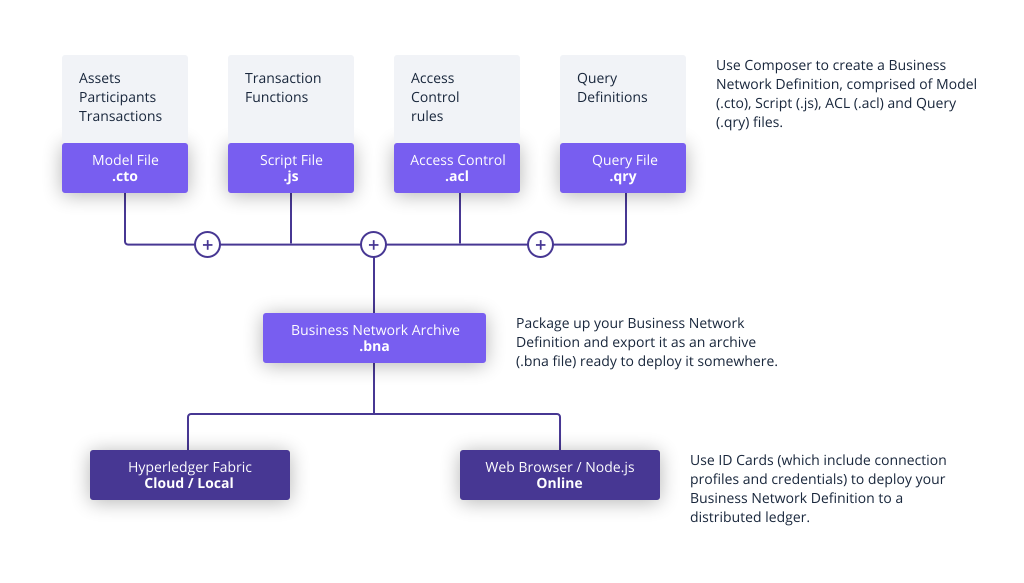
\includegraphics[scale=0.60]{img/composer.png}
			\caption{Implementarea unei re'tele blockchain uitliz\^and Hyperledger Composer}
  			\label{fig:comp}
  		\end{center}
  		\end{figure}
  		
\subsection{MongoDB}
MongoDB\footnote{https://www.mongodb.com/} este o baza de date non-rela'tional'a conceput'a de compania 10gen. Diferen'ta principala fa't'a de bazele de date rela'tionale este in stocarea informa'tiilor nu 'in tabele ci 'in fisiere care utilizeaz'a formatul BSON(binary JSON). Aceste fi'siere sunt organizate sub forma unor colec'tii care sunt similare cu tabele din bazele de date rela'tionale.


\subsection{Loopback}
Loopback\footnote{https://loopback.io/} este un framework Node.js care permite generarea rapida a unui server REST din diferite tipuri de surse de date. Sun disponibili conectori pentru baze de date(SQL, MongoDB) sau pentru o sursa de date precum Hyperledger Composer. Loopback utilizeaza modelul de date scris in Hyperledger Composer pentru a genera operatii CRUD pentru aplicatie si puncte de acces pentru executarea tranzactiilor si a logicii acestora.

\subsection{Passport}
Passport\footnote{http://www.passportjs.org/} este un middleware pentru Node.js av\^and ca scop autentificarea cererilor. Sunt puse la dispozitie diferite stategii de autentificare folosind protocolul OAuth. Printre aceste strategii se numara platforme web populare cum ar fi: Google, Github, etc. Identitatea unui utilizator poate fi stocata fie in cadrul sesiunii uni browser fie in interiorul unui request.
\subsection{OAuth}
OAuth este un framework de autorizare care permite aplica'tiilor s'a limiteze accesul la anumite resurse doar utilizatorilor autentifica'ti, folosind servicii externe sistemului(Google, Github, etc). 

Protocolul OAuth define'ste 4 roluri:
\begin{enumerate}
    \item Resource owner: este utilizatorul care autorizeaz'a accesul la informa'tii legate de contul s'au
    \item Authorization  server: reprezint'a serverul care g'azduie'ste informa'tiile despre contul unui utilizator 'si care expune un API pentru autorizare
    \item Client: aplica'tia care dore'ste sa acceseze informa'tiile legate de contul unui utilizator
    \item Resource server: con'tine resursele accesibile doar utilizatorilor autentifica'ti
\end{enumerate}

	\begin{figure}[H]
		\begin{center}
			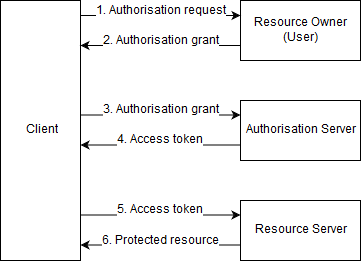
\includegraphics[scale=0.50]{img/oauth.png}
			\caption{Model abstract de func'tionare al protocolului OAuth\cite{oauth}}
  			\label{fig:oauth}
  		\end{center}
  		\end{figure}
  		
Figura \ref{fig:oauth} prezint'a modul de func'tionare al protocolului:
\begin{enumerate}
    \item Aplica'tia trimite o cerere de autorizare serverului care de'tine informa'tii despre utilizator
    \item 'In cazul in care utilizatorul autorizeaz'a cererea aplica'tia prime'ste acces
    \item Aplica'tia cere un token de acces prin prezentarea identit'a'tii utilizatorului 'si a confirm'arii de autorizare
    \item Serverul de autorizare returneaz'a un token de autorizare 'in cazul 'in care informa'tiile trimise de aplica'tie sunt valide
    \item Aplica'tia cere o anumit'a resursa cu acces limitat prin prezentarea token-ului de acces
    \item Serverul de resurse returneaz'a resursa cerut'a 'in cazul 'in care tokenul de acces este valid
    \end{enumerate}




\chapter{Proiectare de Detaliu 'si Implementare}




\chapter{Testare 'si Validare}


\chapter{Manual de Instalare 'si Utilizare}

\chapter{Concluzii}



%\addcontentsline {toc}{chapter}{Bibliography} 
\bibliographystyle{IEEEtran} 
\bibliography{thesis}%same file name as for .bib

%\appendix
\chapter{Profil de conexiune Hyperledger Composer}
\label{app:con}
\begin{verbatim}
{
    "name": "fabric-network",
    "x-type": "hlfv1",
    "version": "1.0.0",
    "peers": {
        "peer0.org1.example.com": {
            "url": "grpc://localhost:7051",
            "eventUrl": "grpc://localhost:7053"
        }
    },
    "certificateAuthorities": {
        "ca.org1.example.com": {
            "url": "http://localhost:7054",
            "caName": "ca.org1.example.com"
        }
    },
    "orderers": {
        "orderer.example.com": {
            "url": "grpc://localhost:7050"
        }
    },
    "organizations": {
        "Org1": {
            "mspid": "Org1MSP",
            "peers": [
                "peer0.org1.example.com"
            ],
            "certificateAuthorities": [
                "ca.org1.example.com"
            ]
        }
    },
    "channels": {
        "composerchannel": {
            "orderers": [
                "orderer.example.com"
            ],
            "peers": {
                "peer0.org1.example.com": {
                    "endorsingPeer": true,
                    "chaincodeQuery": true,
                    "eventSource": true
                }
            }
        }
    },
    "client": {
        "organization": "Org1",
        "connection": {
            "timeout": {
                "peer": {
                    "endorser": "300",
                    "eventHub": "300",
                    "eventReg": "300"
                },
                "orderer": "300"
            }
        }
    }
}
\end{verbatim}

\chapter{Configurare server REST cu utilizatori multiplii}
\label{multiusr}
\begin{verbatim}
export COMPOSER_PROVIDERS='{
  "github": {
    "provider": "github",
    "module": "passport-github",
    "clientID": "[ID]",
    "clientSecret": "[SECRET]",
    "authPath": "/auth/github",
    "callbackURL": "/auth/github/callback",
    "successRedirect": "http://localhost:4200?loggedIn=true",
    "failureRedirect": "/"
  }
}'

export COMPOSER_DATASOURCES='{
    "db": {
        "name": "mydb",
        "connector": "mongodb",
        "database": "mydb",
        "host": "localhost"
    }
}'


composer-rest-server -c admin@clinic-trial-network -n never -m true
\end{verbatim}

\chapter{Modul pentru testarea aplica'tiei client}
\label{app:test}
\begin{verbatim}
describe('OrganisationFormComponent', () => {
  let component: OrganisationFormComponent;
  let fixture: ComponentFixture<OrganisationFormComponent>;

  beforeEach(async(() => {
    TestBed.configureTestingModule({
      imports: [
        FormsModule,
        ReactiveFormsModule,
        AppMaterialModule,
        RouterTestingModule,
        HttpClientModule,
        BrowserAnimationsModule
      ],
      declarations: [OrganisationFormComponent],
      providers:[
        ResearchSiteService,
        SupplyOrganisationService,
        DataService,
        Configuration
      ]
    })
      .compileComponents();
  }));
  beforeEach(() => {
    fixture = TestBed.createComponent(OrganisationFormComponent);
    component = fixture.componentInstance;
    fixture.detectChanges();
  });

  it('should create', () => {
    expect(component).toBeTruthy();
  });
});
\end{verbatim}



\end{document}
